\documentclass{article}

\usepackage[letterpaper]{geometry}
\usepackage{siunitx}
\usepackage{amsmath}
\usepackage{graphicx}
\usepackage{amssymb}

\title{4125 HW 2}
\author{Duncan Wilkie}
\date{3 February 2022}

\begin{document}

\maketitle

\section*{1.34a}
For process A, the volume is constant, so there is no work done on the gas. Therefore, $\Delta U=-Q$. There are five degrees of freedom, all quadratic, for a diatomic molecule with frozen-out vibrational modes; the internal energy is therefore $\frac{5}{2}kT_i$ at the beginning of the process and $\frac{5}{2}kT_f$ at the end. The delta is then, applying the equation of state,
\[\Delta U=\frac{5}{2}k(T_f-T_i)=\frac{5}{2}\left(P_fV_f-P_iV_i \right)=\frac{5}{2}(P_2V_1-P_1V_1)\]
The heat put into the gas is then $Q=\frac{5}{2}(P_2V_1-P_1V_1)$.

For process B, the pressure is constant, so the work done by the gas is the integral $W=-\int PdV$. Since the process is a horizontal line on the $PV$ diagram, this is just the area of the rectangle, i.e. $W=-P(V_f-V_i)=P_2(V_1-V_2)$. The internal energy is the same as above, so the change in it is
\[\Delta U=\frac{5}{2}k(T_f-T_i)=\frac{5}{2}(P_2V_2-P_2V_1)\]
The heat put in the gas is therefore \[Q=\Delta U-W=\frac{5P}{2}(V_f-V_i)-(-P(V_f-V_i))=\frac{7}{2}P_2(V_2-V_1)\]

Processes C and D have the same formulas in terms of initial and final varaibles as processes A and B, just with different values for those variables.
For process C,
\[W=0\textrm{, } \Delta U=\frac{5}{2}(P_1V_2-P_2V_2)\textrm{, } Q=\frac{5}{2}(P_1V_2-P_2V_2)\]
For process D,
\[W=P_1(V_2-V_1)\textrm{, }\Delta U=\frac{5}{2}(P_1V_1-P_1V_2)\textrm{, }Q=\frac{7}{2}P_1(V_1-V_2)\]

\section*{1.34b}
During step A, heat is added to the gas and the piston is held fixed. During step B, the piston is pulled back and heat added so the pressure remains constant. During step C, the piston is held fixed and heat is removed. During step D, the piston is pushed in and heat removed from the gas so the pressure remains constant.

\section*{1.34c}
These net values are just the sums of their values in each case, i.e.
\[W=W_A+W_B+W_C+W_D=0+P_2(V_1-V_2)+0+P_1(V_2-V_1)=-(P_2-P_1)(V_2-V_1)\]
\[\Delta U=\Delta U_A+\Delta U_B+\Delta U_C+\Delta U_D=\frac{5}{2}(P_2V_1-P_1V_1)+\frac{5}{2}(P_2V_2-P_2V_1)+\frac{5}{2}(P_1V_2-P_2V_2)+\frac{5}{2}(P_1V_1-P_1V_2)\]
\[=0\]
\[Q=Q_A+Q_B+Q_C+Q_D=\frac{5}{2}(P_2V_1-P_1V_1)+\frac{7}{2}(P_2V_2-P_2V_1)+\frac{5}{2}(P_1V_2-P_2V_2)+\frac{7}{2}(P_1V_1-P_1V_2)\]
\[=P_1V_1-P_2V_1+P_2V_2-P_1V_2=(P_2-P_1)(V_2-V_1)\]

\section*{1.38}
The process for bubble A is adiabatic, and so satisfies $V=\left( \frac{P_0V_0}{P} \right)^{1/\gamma}$. The process for bubble B is isothermal, and so satisfies $V=\frac{P_0V_0}{P}$. Since $\gamma=1+\frac{2}{f}$, $\gamma > 1$, so an adiabatic process increases in volume faster than an isotherm as pressure decreases. In other words, if an adiabatic and an isothermal process share the same starting point on a $PV$ diagram and pressure decreases, the adiabat will have a greater volume for the same pressure, implying bubble A will be larger at the surface of the lake. A plot of the two $V(P)$ curves with $P_0V_0=1$ and $f=5\Leftrightarrow \gamma=\frac{5}{3}$ appears below for illustration.
\[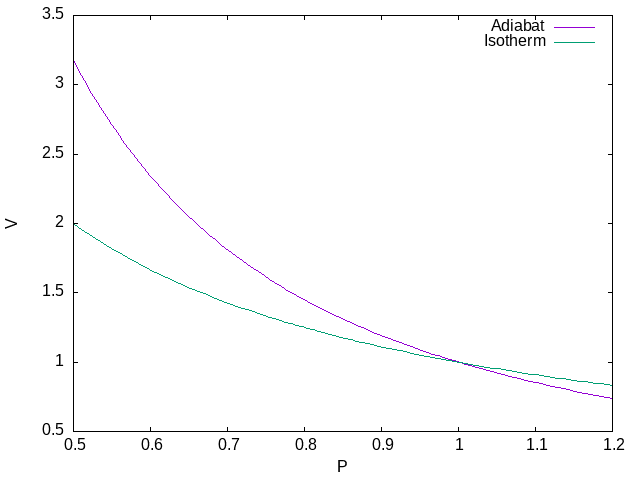
\includegraphics[scale=0.75]{138.png}\]

\section*{1.40a}
The equation of state yields the following expression for temperature:
\[T=\frac{PV}{k}\]
Applying the equation for an adiabat
\[PV^{1+2/f}=P_0V_0\Leftrightarrow V=\left( \frac{P_0V_0}{P} \right)^\frac{1}{1+2/f}\]
we may eliminate V in the equation of state to obtain
\[T(P)=\frac{(P_0V_0)^{1/(1+2/f)}}{kP^{\frac{1}{1+2/f}-1}}\]
Differentiating with respect to $P$,
\[\frac{dT}{dP}=\left( 1-\frac{1}{1+2/f} \right)\frac{(P_0V_0)^{1/(1+2/f)}}{kP^{\frac{1}{1+2/f}-1}P}=\frac{2/f}{1+2/f}\frac{T}{P}=\frac{2}{f+2}\frac{T}{P}\]
as desired.

\section*{1.40b}
Using the chain rule $\frac{dT}{dz}=\frac{dT}{dP}\frac{dP}{dz}$, the temperature gradient is
\[\frac{dT}{dz}=-\frac{2}{f+2}\frac{T}{P}\frac{mg}{kT}P=-\frac{2mg}{k(f+2)}\]

\section*{1.43}
The specific heat of water at constant volume was given in the book as $\SI{4.2}{J/g^\circ C }$. The atomic mass of a water molecule is \SI{18}{amu}, so about 18 grams of water corresponds to one mole. The heat capacity per molecule is then
\[\frac{C}{N}\frac{(\SI{18}{g})(\SI{4.2}{J/g^\circ C})}{\SI{6.02e23}{}}=\SI{1.26e-22}{J/^\circ C}=9.1k\]
The equipartition theorem suggests that, presuming all degrees of freedom are quadratic, this number is equal to $\frac{f}{2}k$, since multiplying by the total number of particles and a temperature would yield the internal energy of the water. This suggests the water molecule has around 18 degrees of freedom, which seems a little absurd.

\section*{1.48}
The power density actually absorbed by the snow pack is $0.1(\SI{1}{kW/m^2})=\SI{100}{W/m^2}$. In a square meter of the snow pack, there is a total volume of $\SI{2}{m^3}$. Half of this is ice, so one cubic meter of ice is present. The density of ice is $\SI{919}{kg/m^3}$ according to a table I found online. If the ice is already at \SI{32}{^\circ C}, the amount of energy required to melt it using the latent heat of fusion given in the book of $\SI{333}{J/g}=\SI{333}{kJ/kg}$ is
\[Q=Lm={(\SI{333}{kJ/kg})}{(\SI{919}{kg/m^3})}=\SI{306}{MJ}\]
Dividing this by the power the snow absorbs, it would take
\[t=\frac{Q}{P}=\frac{\SI{306e6}{J}}{\SI{100}{W/m^2}}=\SI{3.06e6}{s}\approx \SI{35.4}{days}\]
of constant sunshine. A more reasonable estimate would be a 12-hour daylight period, which would double the necessary time to 71 days.

\section*{1.49}
The work required to displace the 1.5 moles of ideal gas, and therefore the work done by the atmosphere, is
\[PV={nRT}={(\SI{1.5}{mol})(\SI{8.31}{J/mol\cdot K})(\SI{300}{K})}=\SI{3740}{J}\]
The rest of the heat energy is generated by the reaction, specifically the other $\SI{286}{kJ}-\SI{3.74}{kJ}=\SI{282}{kJ}$

\section*{1.54a}
The amount of work needed is
\[W=mgh=(\SI{60}{kg})(\SI{9.81}{m/s^2})(\SI{1500}{m})=\SI{883}{kJ}\]
This value is 25\% of the value she needs to consume, so she needs to eat
\[\frac{\SI{883}{kJ}}{0.25}=\SI{3.53}{MJ}=\SI{844}{kcal}\]
She therefore needs roughly 8.5 bowls of cornflakes.

\section*{1.54b}
Since the body is mostly water, we'll approximate it by treating it as entirely water. The change in temperature would be
\[\Delta T=\frac{\Delta U}{mc_V}=\frac{(0.75)(\SI{3.53e3}{kJ})}{(\SI{4.2}{kJ/kg^\circ C})(\SI{60}{kg})}=\SI{10.5}{^\circ C}\]

\section*{1.54c}
The amount of water evaporated may be found using the latent heat of evaporation given in the book from
\[m=\frac{Q}{L}=\frac{(0.75)(\SI{3.53e3}{kJ})}{\SI{2428}{kJ/kg}}=\SI{1.1}{kg}\]
Water is almost exactly one gram per milliliter, so she should drink about $\SI{1.1}{L}$.

\section{}
Using the equation of state,
\[ V=\frac{N_1k T_1}{P},\]
\[V=\frac{N_2 k T_2}{ P}\]
Since the molar mass of hydrogen is \SI{2}{g/mol}, $\SI{6}{kg}$ of hydrogen corresponds to \SI{3000}{mol} or $\SI{1.81e27}{molecules}$.
Substituting,
\[V=\frac{(N_1-\SI{1.81e27}{})kT_2}{P},\]
\[V=\frac{N_1kT_1}{P}\]
This is a system of two equations and two unknowns; eliminating $N_1$ in the first by writing the second as
\[N_1=\frac{VP}{kT_1}\]
yields
\[V=\frac{(VP/kT_1-\SI{1.81e27}{})kT_2}{P}=V\frac{T_2}{T_1}-\frac{(\SI{1.81e27}{})kT_2}{P}\]
\[\Leftrightarrow V=-\frac{(\SI{1.81e27})kT_2}{P(1-\frac{T_2}{T_1})}=-\frac{(\SI{1.81e27})(\SI{1.38e-23}{J/K})(\SI{310}{K})}{(\SI{1.01e6}{Pa})(1-\frac{\SI{310}{K}}{\SI{288}{K}})}=\SI{100}{m}\]

\section{}
Isothermal compression implies no change in the internal energy, since $U\propto T$ Therefore, the the heat is $Q=-W$ by the first law of thermodynamics. Isotherms on a $PV$ plot are given by \[PV=P_0V_0\Leftrightarrow P=\frac{P_0V_0}{V}=\frac{NkT_0}{V}\]
The corresponding work is
\[W=-\int_{V_0}^{V_1}P(V)dV=-\int_{V_0}^{V_1}\frac{NkT_0}{V}dV=NkT_0\ln\left( \frac{V_0}{V_1} \right)=NkT_0\ln\left( \frac{P_1}{P_0} \right)\]
Diatomic nitrogen's molar mass is $\SI{28}{g/mol}$, so this is a quarter mole of nitrogen, or $(0.25)(\SI{6.02e23})=\SI{1.51e23}{molecules}$.
Plugging in the values,
\[Q=-W=NkT\ln\left( \frac{P_0}{P_1} \right)=(\SI{1.51e23}{})(\SI{1.38e-23}{J/K})(\SI{300}{K})\ln\left( \frac{\SI{1.01e6}{Pa}}{\SI{50.50e6}{Pa}} \right)=-\SI{2446}{J}\]
The form of the first law used presumes this is heat given to the gas, so there is this much heat released. The work found is the negative of the above number by construction, and is taken to be the work done on the gas by an external agent.

\section{}
The work done under such a process is
\[W=-\int_{V_0}^{V_1}P(V)dV=-\int_{V_0}^{V_1}\sqrt{\frac{P_0^2V_0}{V}}dV=-P_0\sqrt{V_0}\left( 2\sqrt{V}\bigg|_{V_0}^{V_1} \right)=2P_0V_0^{3/2}-2P_0\sqrt{V_0V_1}\]
Using the definition of the process,
\[=2P_0V_0^{3/2}-2P_0V_0\frac{P_0V_0}{P_1}=2P_0V_0^{3/2}-2\frac{P_0^2V_0^2}{P_1}\]

The heat capacity under this process is therefore
\[C=\frac{\Delta U}{\Delta T} - \frac{\Delta W}{\Delta T}=\frac{Nfk}{2}+2P_0^2V_0^2\frac{d}{d T}\frac{V_1}{NkT}\]
\[=\frac{Nfk}{2}+2P_0^2V_0^2\left( \frac{1}{NkT}\frac{\partial V_1}{\partial T}-\frac{V_1}{NkT^2} \right)\]
\[=\frac{Nfk}{2}+2P_0^2V_0^2\left( \frac{1}{P_1T}- \frac{1}{P_1T}\right)\]
\[=\frac{Nfk}{2}\]
It then follows that the heat capacity for $n$ moles is $n\frac{N_Afk}{2}$

\section{}
Nitrogen is a diatomic gas, and so has five degrees of freedom presuming temperatures sufficiently reasonable to freeze out the vibrational modes. Therefore, $\gamma=1+\frac{2}{f}=\frac{7}{5}$. The heat transferred to the gas is by assumption of adiabaticity zero, so we only need to calculate the work; this is done by
\[W=-\int_{V_0}^{V_1}P(V)dV=-\int_{V_0}^{V_1}\frac{P_0V_0}{V^{7/2}}dV=\frac{2P_0V_0}{5V^{5/2}}\bigg|_{V_0}^{V_1}=\frac{2P_0V_0}{5}\left( \frac{1}{V_1^{5/2}}-\frac{1}{V_0^{5/2}} \right)\]
This is equal to the change in internal energy by the first law of thermodynamics. Evaluating,
\[\Delta U=\frac{2(\SI{1.01e6}{Pa})(\SI{0.01}{m^3})}{5}\left( \frac{1}{(\SI{0.32}{m^3})^{5/2}}-\frac{1}{(\SI{0.01}{m^3})^{5/2}} \right)=\SI{-404}{MJ}\]



\end{document}
%%% Local Variables:
%%% mode: latex
%%% TeX-master: t
%%% End:
